\documentclass[a4paper,11pt]{article}
\usepackage{cite}
\usepackage[svgnames]{xcolor}
\usepackage{tikz}
\usetikzlibrary{arrows.meta, patterns, angles, calc, positioning}
\tikzset{ x=1cm, y=1cm, >=Latex, Ap/.style={draw, solid, <-, shorten <=2pt, angle radius=#1cm, angle eccentricity=1.1} }
\def\myR{1} \def\myangle{70}
\bibliographystyle{IEEEtran}


% argument is your BibTeX string definitions and bibliography database(s)

\bibliography{IEEEabrv,citation.bib}
\bibliographystyle{plain}
\bibliography{ref}
% define the title
\author{H.~Partl}
\title{Minimalism}
\begin{document}
% generates the title
\maketitle
% insert the table of contents
\tableofcontents
\section{Some Interesting Words}
Well, and here begins my lovely article.
\section{Good Bye World}
\ldots{} and here it ends.

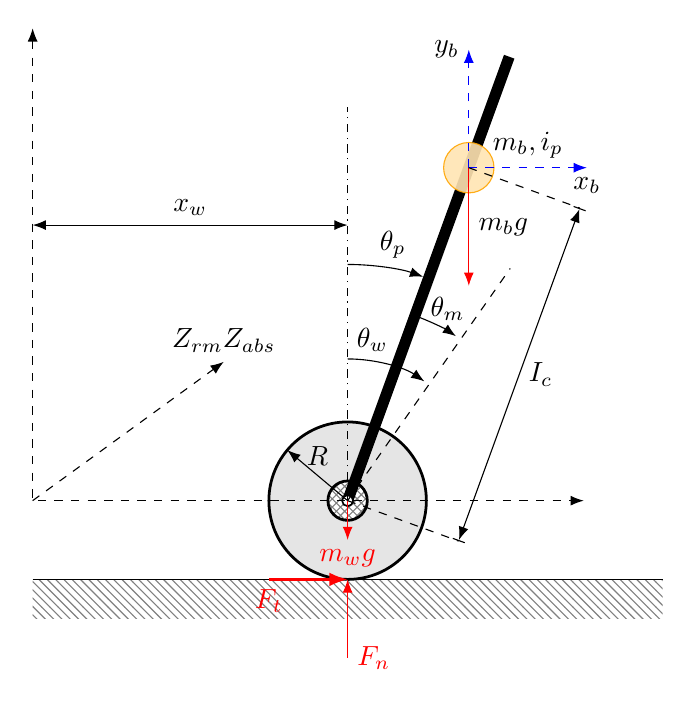
\begin{tikzpicture}
\draw[line width=1pt, fill=gray!20] (0,0) coordinate(O) circle[radius=\myR];
\draw[fill=white] (O) circle[radius=\myR*0.25];
\draw[line width=1pt, pattern=crosshatch, pattern color=gray] (O) circle[radius=\myR*0.25];
\draw[line width=4pt] (O)--(\myangle:6) coordinate (B);
\draw[line width=0.6pt, fill=white] (O) circle[radius=2pt];
\draw[dash dot] (O) -- (0,5) coordinate (A);
\draw[dashed] (O) -- (55:3.6) coordinate (C) 
      pic[pic text={$\theta _p$}, Ap=3]{angle=B--O--A}
      pic[Ap=1.8]{angle=C--O--A} node[above] at (80:1.8) {$\theta _w$}
      pic[pic text={$\theta _{m}$}, Ap=2.5] {angle=C--O--B};
\draw[->] (O) -- node[midway, above]{$R$} (140:\myR);
\coordinate (O2) at (\myangle:4.5);
\draw[fill=Orange!30, opacity=0.9, draw=Orange] (O2) circle[radius=\myR*0.32];
\draw[->, draw=Blue, dashed] (O2)--+(0,1.5)node[left]{$y_b$}; \draw[->, draw=Blue, dashed] (O2)-- node[midway, above]{$m_b,i_p$} +(1.5,0) node[below]{$x_b$};
\draw[->, draw=Red] (O2) -- node[midway, right]{$m_bg$} +(0,-1.5);
\draw[dashed] (O) -- +(\myangle-90:1.5) coordinate(a) (O2) -- +(\myangle-90:1.5) coordinate(b);
\draw[|<->|] (a)-- node[midway, right]{$I_c$} (b);
\draw[dashed, <->] (-4,6)--(-4,0) coordinate(O3)--(3,0); 
\draw[dashed, ->] (O3)--+(36:3) node[above]{$Z_{rm}Z_{abs}$};
\draw[<->] (-4,3.5)-- node[midway,above]{$x_w$} (0,3.5);
\path[pattern=north west lines, pattern color=gray] (-4,-\myR) -- (4,-\myR) -- ++(0,-0.5) -- ++(-8,0)--cycle;
\draw (-4,-\myR) -- (4,-\myR);
\draw[Red, ->] (O) -- +(0,-0.5) node[below]{$m_wg$};
\draw[Red, <-] (0,-\myR) -- +(0,-1) node[right]{$F_n$};
\draw[Red, <-, thick] (0,-\myR) -- +(-1,0) node[below]{$F_t$};
\end{tikzpicture}
% 设置标注
\footnote{this is a foot note}



\end{document}
@ARTICLE{2018arXiv180400092W,
       author = {{Wang}, Yisen and {Liu}, Weiyang and {Ma}, Xingjun and {Bailey}, James and {Zha}, Hongyuan and {Song}, Le and {Xia}, Shu-Tao},
        title = "{Iterative Learning with Open-set Noisy Labels}",
      journal = {arXiv e-prints},
     keywords = {Computer Science - Computer Vision and Pattern Recognition},
         year = 2018,
        month = mar,
          eid = {arXiv:1804.00092},
        pages = {arXiv:1804.00092},
archivePrefix = {arXiv},
       eprint = {1804.00092},
 primaryClass = {cs.CV},
       adsurl = {https://ui.adsabs.harvard.edu/abs/2018arXiv180400092W},
      adsnote = {Provided by the SAO/NASA Astrophysics Data System}
}


